% figures/stage-gate.tex
% Standalone TikZ: Stage-Gate NPD process — five stages with Go/Kill/Hold decision diamonds.
\documentclass[tikz,border=6pt]{standalone}
\usepackage{tikz}
\usetikzlibrary{arrows.meta,positioning,calc,shapes.geometric}

\definecolor{vcblue}{HTML}{1A5276}
\definecolor{vcteal}{HTML}{0E6655}
\definecolor{vcgrey}{HTML}{5D6D7E}
\definecolor{vcred}{HTML}{7B241C}

\begin{document}
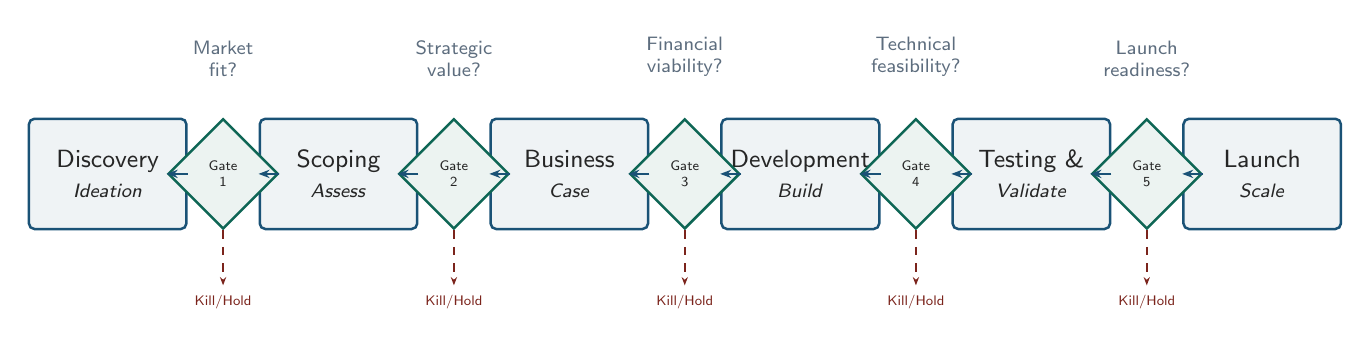
\begin{tikzpicture}[
  node distance=6mm and 5mm,
  stage/.style={
    draw=vcblue, line width=0.9pt, rounded corners=2pt, fill=vcblue!7,
    font=\sffamily\small, align=center,
    minimum width=20mm, minimum height=14mm, text=black!85},
  gate/.style={
    diamond, draw=vcteal, line width=0.9pt, fill=vcteal!8,
    font=\sffamily\tiny, align=center,
    minimum width=14mm, minimum height=14mm,
    inner sep=1pt, text=black!85,
    aspect=1},
  arrow/.style={-{Stealth[length=4pt]}, vcblue, line width=0.9pt},
  kill/.style={-{Stealth[length=3pt]}, vcred, line width=0.7pt, dashed},
  ann/.style={font=\sffamily\scriptsize, text=vcgrey, align=center},
]

  %% ---- Stages ----
  \node[stage] (disc)  {Discovery\\{\scriptsize\textit{Ideation}}};
  \node[stage, right=9mm of disc]  (scope) {Scoping\\{\scriptsize\textit{Assess}}};
  \node[stage, right=9mm of scope] (bcase) {Business\\{\scriptsize\textit{Case}}};
  \node[stage, right=9mm of bcase] (dev)   {Development\\{\scriptsize\textit{Build}}};
  \node[stage, right=9mm of dev]   (test)  {Testing \&\\{\scriptsize\textit{Validate}}};
  \node[stage, right=9mm of test]  (laun)  {Launch\\{\scriptsize\textit{Scale}}};

  %% ---- Gates (positioned midway between stages) ----
  \node[gate] (g1) at ($(disc.east)!0.5!(scope.west)$) {Gate\\1};
  \node[gate] (g2) at ($(scope.east)!0.5!(bcase.west)$) {Gate\\2};
  \node[gate] (g3) at ($(bcase.east)!0.5!(dev.west)$)   {Gate\\3};
  \node[gate] (g4) at ($(dev.east)!0.5!(test.west)$)    {Gate\\4};
  \node[gate] (g5) at ($(test.east)!0.5!(laun.west)$)   {Gate\\5};

  %% ---- Forward flow ----
  \draw[arrow] (disc.east)  -- (g1.west);
  \draw[arrow] (g1.east)    -- (scope.west);
  \draw[arrow] (scope.east) -- (g2.west);
  \draw[arrow] (g2.east)    -- (bcase.west);
  \draw[arrow] (bcase.east) -- (g3.west);
  \draw[arrow] (g3.east)    -- (dev.west);
  \draw[arrow] (dev.east)   -- (g4.west);
  \draw[arrow] (g4.east)    -- (test.west);
  \draw[arrow] (test.east)  -- (g5.west);
  \draw[arrow] (g5.east)    -- (laun.west);

  %% ---- Kill / Hold exits (downward from each gate) ----
  \foreach \g/\lbl in {g1/{Kill/Hold},g2/{Kill/Hold},g3/{Kill/Hold},g4/{Kill/Hold},g5/{Kill/Hold}}{
    \draw[kill] (\g.south) -- ++(0,-7mm)
      node[below, font=\sffamily\tiny, text=vcred, align=center] {\lbl};
  }

  %% ---- Gate criterion annotations (above each gate) ----
  \node[ann, above=4mm of g1] {Market\\fit?};
  \node[ann, above=4mm of g2] {Strategic\\value?};
  \node[ann, above=4mm of g3] {Financial\\viability?};
  \node[ann, above=4mm of g4] {Technical\\feasibility?};
  \node[ann, above=4mm of g5] {Launch\\readiness?};

\end{tikzpicture}
\end{document}
